\documentclass[12pt]{article}
\usepackage{amsmath,amssymb,amsthm}
\usepackage{graphicx}
\usepackage{float}
\usepackage{hyperref}
\topmargin=-45pt  
\headheight=12truept 
\headsep=25pt
\footskip=37pt 
\hoffset=0pt 
\voffset=12pt
\oddsidemargin=0cm 
\evensidemargin=0cm
\textheight=23.7cm 
\textwidth=16.0cm

\def \nequiv {\equiv \hspace{-3mm} / \hspace{1mm}}
\def \qed {\hfill \hbox {\rule [-2pt]{3pt}{6pt}}}
%\pagestyle{myheadings}
%%%%%%%%%%%%%
\newtheorem{thm}{Theorem}%[chapter]% THEOREM
\newtheorem{theorem}[thm]{Theorem}
\newtheorem{prop}[thm]{Proposition}% PROPOSITION
\newtheorem{proposition}[thm]{Proposition}
\newtheorem{cor}[thm]{Corollary}% COROLLARY
\newtheorem{corollary}[thm]{Corollary}
\newtheorem{lem}[thm]{Lemma}% LEMMA
\newtheorem{lemma}[thm]{Lemma}
\newtheorem{remark}[thm]{Remark}
\newtheorem{defi}[thm]{Definition}
\newtheorem{definition}[thm]{Definition}
%\newtheorem{example}[thm]{Example}

\begin{document}
\title{Optimal Execution Strategies Incorporating Internal Liquidity Through Market Making}

%\author{
%Yusuke MORIMOTO
%\thanks{
%MUFG Bank, Ltd, 1-4-5 Marunouchi, Chiyoda-ku, Tokyo 100-8388, Japan, \
%E-mail: yuusuke.morimoto@gmail.com} }
\date{}
\maketitle
\begin{abstract}
This paper proposes a novel algorithmic execution model that integrates interbank limit and market orders with internal liquidity provided through market making. 
Building upon a widely used framework for optimal execution, the model incorporates market impact for interbank orders while excluding it for internal market-making executions. The objective is to optimize the allocation between interbank and internal liquidity, thereby reducing market impact and enhancing execution efficiency.
\end{abstract}

JEL Classification: C41, G11
Mathematical Subject Classification (2010): 65C05, 60G40
Keywords: Algorithmic Trading, Market Impact, Optimal Execution, Liquidation, Stochastic Control, Impulse Control

\section{Introduction}

When executing large orders, rapid execution over a short period may trigger unfavorable price movements through market impact. 
Conversely, executing orders too slowly exposes the trader to market risk arising from price fluctuations. 
Optimal execution problems therefore involve a trade-off between market impact costs and inventory risk, and constructing efficient execution strategies has become an important topic in quantitative finance.

The seminal works of Almgren and Chriss \cite{almgren2001optimal} and Bertsimas and Lo \cite{bertsimas1998optimal} introduced foundational frameworks for optimal execution under market impact. 
These studies modeled the asset price as a diffusion process and derived optimal execution strategies using stochastic control and variational methods. 
Since then, many extensions have been proposed, including models with nonlinear market impact, transient impact, and resilience effects 
\cite{dang2017optimal,gatheral2011exponential,gatheral2012transient,curato2017optimal}.

In practical markets, execution is carried out not only through market orders (MOs) but also through limit orders (LOs). 
Consequently, optimal execution models must incorporate bid-offer spreads and the trade-off between aggressive and passive execution methods. 
Cartea et al.~\cite{cartea2015algorithmic} and Cartea and Jaimungal \cite{cartea2015optimal} developed dynamic optimal execution models combining MOs and LOs. 
In their framework, limit-order executions are modeled through Poisson arrivals, while market orders are represented within an impulse-control framework. 
The resulting optimization problem is characterized through a Hamilton--Jacobi--Bellman quasi-variational inequality (HJB-QVI).

While most classical optimal execution models focus primarily on external liquidity, dealer markets and OTC markets increasingly rely on internal liquidity generated through client flow and market-making activity. 
Large financial institutions commonly operate both algorithmic execution services and market-making businesses simultaneously. 
Through market-making operations, internal liquidity is continuously generated from client order flow. 
Such internal liquidity can potentially be utilized within algorithmic execution, thereby reducing the need to execute directly in external markets and mitigating market impact costs.

The importance of internalization and internal liquidity utilization has increased significantly in modern dealer markets. 
In particular, internal execution mechanisms allow institutions to match flows internally rather than routing all transactions to external markets. 
Such mechanisms are expected to improve execution efficiency while reducing market impact and transaction costs. 
These practices are especially important in OTC markets such as foreign exchange markets, although similar structures are also observed in various dealer-driven markets.

There exists extensive research on market making itself, including Avellaneda and Stoikov \cite{avellaneda2008high}, Gu\'eant et al.~\cite{gueant2013dealing}, and Cartea et al.~\cite{cartea2017algorithmic}. 
These studies primarily focus on the optimization of quoting strategies and inventory management for market makers. 
In contrast, most optimal execution studies focus mainly on external liquidity and do not explicitly incorporate internal liquidity generated through market-making activity into the execution framework. 
To the best of our knowledge, there has been limited research integrating market orders, limit orders, and internal market-making executions within a unified optimal execution framework.

The present work proposes an optimal execution model that incorporates not only interbank market orders and limit orders, but also internal liquidity generated through market making as an additional execution source. 
In particular, the proposed model simultaneously incorporates
(i) market orders,
(ii) limit orders,
and
(iii) internal executions through market making,
while distinguishing between external executions with market impact and internal executions without direct market impact.

The primary objective of the proposed framework is to analyze the optimal allocation between external liquidity and internal liquidity. 
In addition, the model allows us to determine how aggressively internal quotes should be provided from the perspective of execution quality. 
This viewpoint differs from the traditional market-making literature, which mainly focuses on the profitability of the market maker itself. 
Instead, the present work focuses on improving execution quality for algorithmic execution clients through the utilization of internal liquidity.

The main contributions of this paper are summarized as follows.
First, we formulate a unified stochastic control and impulse-control framework incorporating market orders, limit orders, and internal market-making executions. 
Second, we derive the corresponding HJB-QVI and characterize the value function within the viscosity-solution framework. 
Third, we perform numerical experiments and sensitivity analyses to investigate how internal liquidity affects optimal execution strategies and execution values. 
The numerical results demonstrate that the availability of internal liquidity significantly improves execution performance and reduces effective market impact costs.

The remainder of this paper is organized as follows.
Section~2 explains the practical mechanism underlying algorithmic execution utilizing market-making liquidity. 
Section~3 introduces the mathematical model and derives the associated HJB-QVI. 
Section~4 presents numerical experiments and sensitivity analyses of the optimal strategies. 
Finally, Section~5 concludes the paper.

\section{Practical Background and Internal Liquidity Mechanism}

This section explains the practical mechanism motivating the proposed model. 
In dealer markets and OTC markets, financial institutions often operate both algorithmic execution services and market-making businesses simultaneously. 
The proposed framework is motivated by the possibility of utilizing internal liquidity generated through market-making activity within algorithmic execution.

Financial institutions operate both as market makers and market takers. 
As market makers, they provide liquidity to clients by continuously quoting bid and ask prices. 
The resulting inventory positions are typically hedged in external interbank markets, where the institution acts as a market taker. 
At the same time, many financial institutions also provide algorithmic execution services, in which large client orders are executed through external markets using market orders or limit orders.

In standard algorithmic execution, client orders are generally executed directly in external markets through combinations of market orders and limit orders. 
However, when a financial institution simultaneously operates a market-making business, internal client flow generated through market making may provide an additional execution opportunity. 
By slightly improving quoted prices for market-making clients, the institution may attract offsetting client flow internally. 
Such internally matched flow can then be utilized by the algorithmic execution desk, thereby reducing the amount of execution required in external markets.

This mechanism can provide benefits for both sides of the transaction. 
Clients using algorithmic execution services may achieve execution at prices more favorable than direct execution in external markets while reducing market impact costs. 
At the same time, clients interacting with the market-making desk may also receive competitive quoted prices. 
As a result, internalization mechanisms have become widely utilized in practice, particularly in OTC markets such as foreign exchange markets.

Figure~\ref{fig:mm} illustrates a typical example of algorithmic execution utilizing internal market-making liquidity in an OTC FX market. 
The execution agent receives a sell order from a client and coordinates with the internal market-making desk to attract offsetting client flow through favorable pricing. 
As a result, internal execution can be achieved at prices more favorable than direct execution in the interbank market, while simultaneously reducing market impact costs.

The figure highlights the following points:
\begin{itemize}
  \item The example considers an OTC FX market such as USD/JPY.
  \item The algorithmic execution client submits a sell order.
  \item The execution desk requests the internal market-making desk to provide favorable quotes in order to attract offsetting client flow.
  \item Clients interacting with the market-making desk can purchase at prices lower than the usual ask price.
  \item The execution desk can reduce market impact by utilizing internally generated liquidity instead of relying entirely on external interbank execution.
\end{itemize}

\begin{figure}[H]
  \centering
  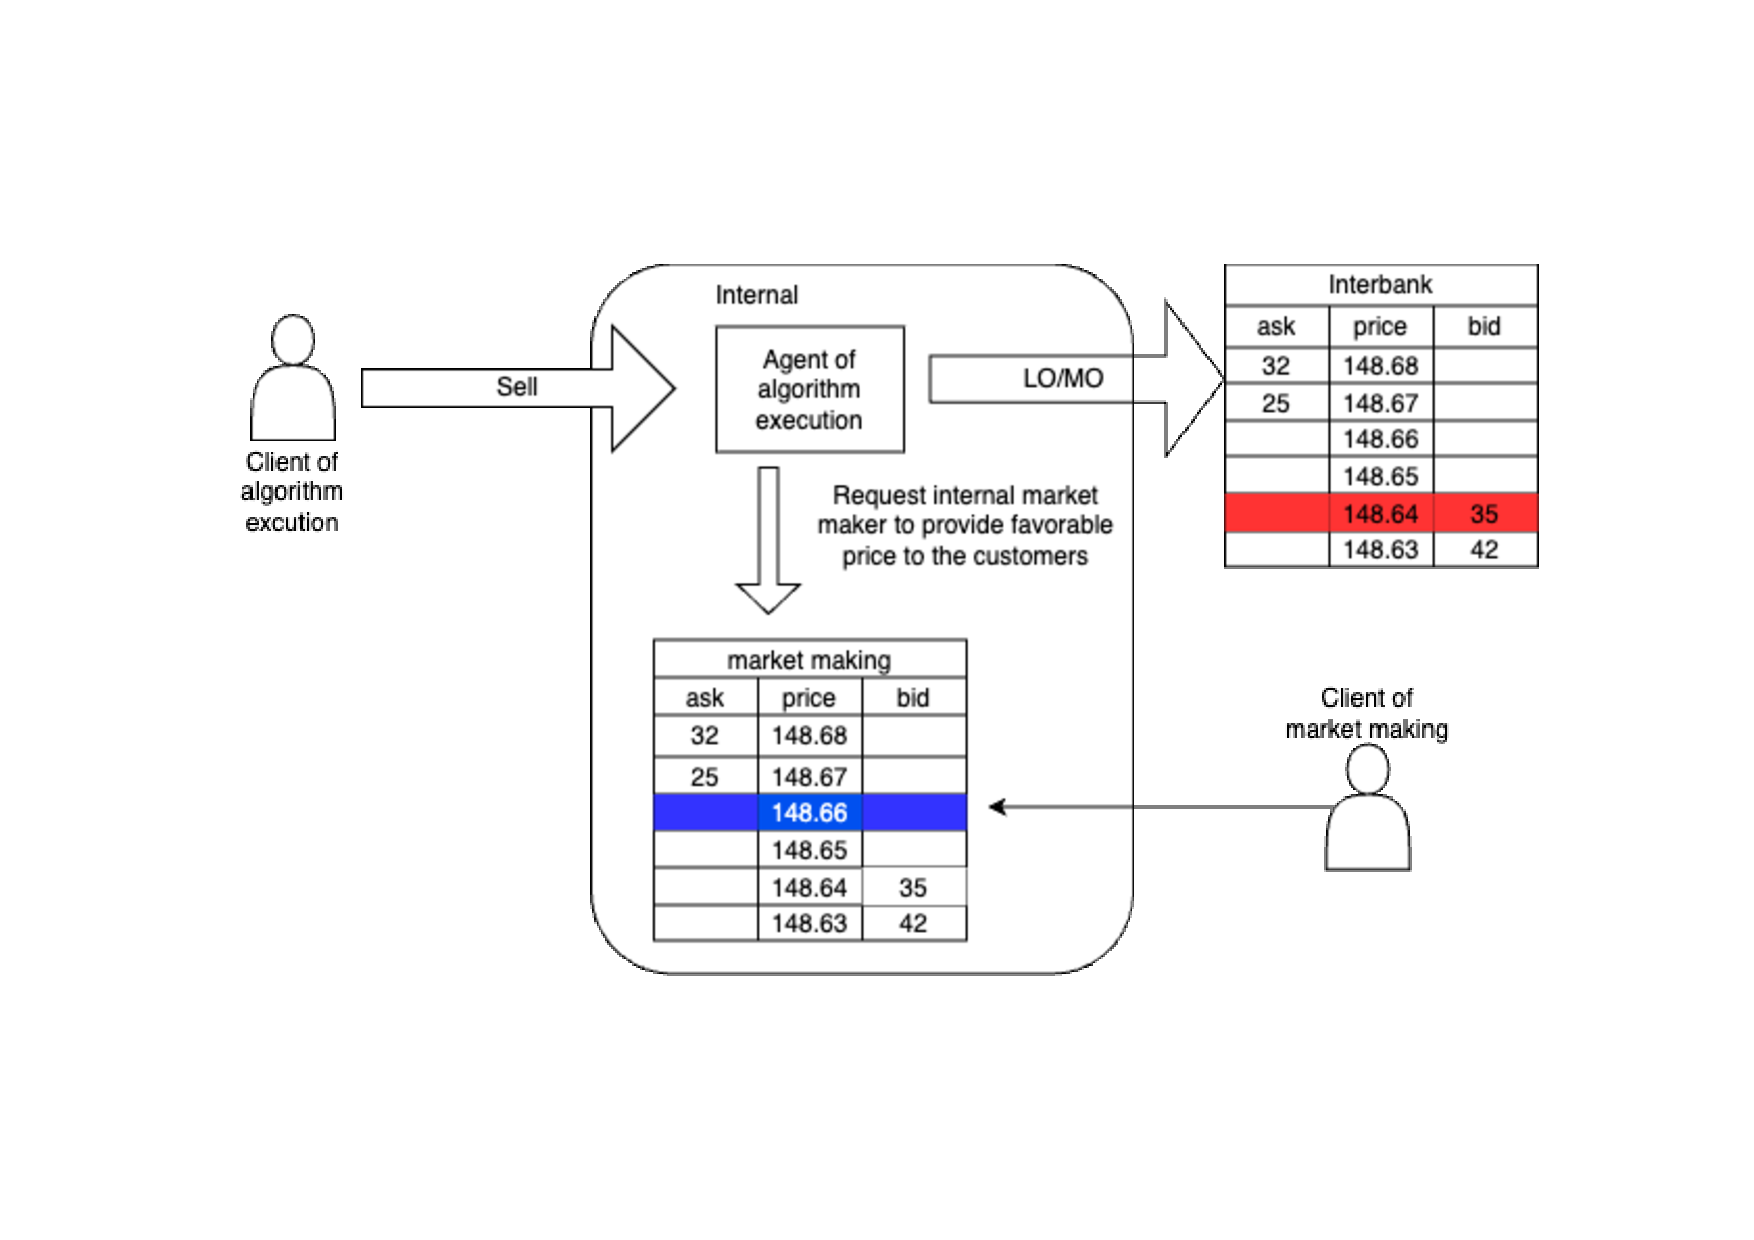
\includegraphics[width=1.0\textwidth]{internal_match.pdf}
  \caption{Illustration of algorithmic execution utilizing internal market-making liquidity}
  \label{fig:mm}
\end{figure}

\section{Model}\label{sec:model}
\subsection{Mathematical Framework: Combined Stochastic Control and Impulse Control}\label{sec:math}
The proposed execution problem combines continuous stochastic controls, corresponding to the choice of spreads for limit and internal market-making orders, together with impulse controls representing market-order executions. 
Such problems naturally fall into the framework of combined stochastic and impulse control problems studied in \O{}ksendal and Sulem \cite{oksendal2019stochastic} and Seydel \cite{seydel2009existence}. 
In particular, the associated value function is characterized through a Hamilton--Jacobi--Bellman quasi-variational inequality (HJB-QVI) in the viscosity solution framework.

In this section, we summarize the standard framework for combined stochastic and impulse control problems developed in Seydel \cite{seydel2009existence}, which provides the theoretical foundation for the HJB-QVI formulation used in this paper.

Let $(\Omega,\mathcal F,\{\mathcal{F}_t\}_{t\in [0, T]},P)$ be a filtered probability space satisfying the usual conditions.
Let $A$ be a compact non-empty metric space. 
The stochastic control process 
\[
v:[0,T]\times\Omega\to A
\]
is assumed to be $\{\mathcal{F}_t\}$-predictable.
Let $W$ be a $d_1$-dimensional $\{\mathcal{F}_t\}$-Brownian motion. 
Let $N$ be a $d_2$-dimensional counting process with compensator
\[
\int_0^t \lambda(v_u)\,du,
\]
where
\[
\lambda : A \to \mathbb{R}_{\ge0}^{d_2}
\]
is a continuous function.
More precisely,
\[
N_t
-
\int_0^t
\lambda(v_u)\,du
\]
is assumed to be a
$\{\mathcal F_t\}$-martingale.

The impulse control is represented by a sequence
\[
\theta=\{(\tau_i,\zeta_i)\}_{i\ge1},
\]
where $\tau_i$ are $\{\mathcal F_t\}$-stopping times and $\zeta_i$ are $\mathcal F_{\tau_i}$-measurable intervention variables taking values in a compact intervention set $\mathcal Z$.

The $k$-dimensional state process $Y$ follows the stochastic differential equation with impulses
\begin{align}\label{eq:sde}
  &dY_t = \mu(Y_{t-}, v_{t-})dt + \sigma(Y_{t-}, v_{t-}) dW_t + \nu(Y_{t-}, v_{t-})dN_t, t \in (\tau_{i-1}, \tau_{i}), \\
  &Y(\tau_i) = \Gamma(\check{Y}(\tau_i-), \zeta_i), i = 1, 2, \cdots, 
\end{align}
where the term $\check{Y}_{\tau_i-}$ denotes the value of the controlled $Y$ in ${\tau_i}$ with a possible jump of the
stochastic process, but without the impulse, i.e., $Y_{\tau_i-} + \Delta Y_{\tau_i}$, \ $\Gamma: {\bf R}^k \times \mathcal{Z} \rightarrow {\bf R}^k, \mu: {\bf R}^k \times A \rightarrow {\bf R}^k, \sigma: {\bf R}^k \times A \rightarrow {\bf R}^{k\times d_1}$ and $\nu: {\bf R}^k \times A \rightarrow {\bf R}^{k\times d_2}$
satisfying the necessary conditions such that existence and uniqueness of the SDE (\ref{eq:sde}) with an initial value $y \in \textbf{R}^k$ is guaranteed.

Let $\mathcal{A}(s,y)$ denote the set of admissible combined stochastic and impulse controls $(v,\theta)$ for which the controlled state process \eqref{eq:sde} is well defined and existence and uniqueness are guaranteed.
For a sufficiently smooth function $\psi$, define the intervention operator
\[
\mathcal{M}\psi(y)
=
\sup_{\zeta\in\mathcal Z}
\psi(\Gamma(y,\zeta)).
\]

The infinitesimal generator associated with the controlled dynamics between interventions is given by
\[
L^v\psi(y)
=
\mu(y,v)\partial_y\psi(y)
+
\frac{1}{2}\sigma(y,v)^2\partial_{yy}\psi(y)
+
\bigl(
\psi(y+\nu(y,v))
-
\psi(y)
\bigr)
\lambda(t,y,v).
\]

We consider the value function
\begin{align}\label{eq:valGen}
H(t,y)
=
\sup_{(v,\theta)\in\mathcal A(t,y)}
E\left[
g(Y_T)
+
\int_t^T
f(u,Y_u,v_u)\,du
\middle|
\mathcal F_t
\right],
\end{align}
where
\[
f:{\bf R}^+\times{\bf R}^k\times A\to{\bf R},
\qquad
g:{\bf R}^k\to{\bf R}
\]
are measurable reward functions.

According to the dynamic programming principle for combined stochastic and impulse control problems, we introduce the following formal HJB-QVI associated with the value function.
\begin{definition}[Formal HJB-QVI]
  The formal Hamilton--Jacobi--Bellman quasi-variational inequality associated with the value function \eqref{eq:valGen}
\begin{align}
\max\left\{
\partial_tH(t,y)
+
\sup_{v\in A}
\bigl(
L^vH(t,y)
+
f(t,y,v)
\bigr),
\mathcal{M}H(t,y)-H(t,y)
\right\}
=
0,
\label{HJBQVI}
\end{align}
with terminal condition
\[
H(T,y)=g(y).
\]
\end{definition}

Following Seydel \cite{seydel2009existence},
we impose the following assumptions on the controlled dynamics and reward functions.

\begin{enumerate}
\item[(A1)]
The stochastic control set $A$ and intervention set $\mathcal Z$ are compact.

\item[(A2)]
The coefficients
\[
\mu,\sigma,\nu,\Gamma,\lambda
\]
are continuous in the state and control variables and satisfy standard continuity and growth conditions ensuring existence and uniqueness of the controlled process.

\item[(A3)]
The reward functions
\[
f(t,y,v),
\qquad
g(y)
\]
are continuous and satisfy polynomial growth conditions.

\item[(A4)]
The associated HJB-QVI admits a comparison principle within the corresponding growth class.
\end{enumerate}
The following theorem summarizes Theorem 2.2 of Seydel \cite{seydel2009existence}.
\begin{theorem}[Seydel \cite{seydel2009existence}]
\label{thm:seydel}
Suppose that assumptions (A1)--(A4) hold.
Then the value function
\[
H(t,y)
=
\sup_{(v,\theta)\in\mathcal A(t,y)}
E\left[
g(Y_T)
+
\int_t^T
f(u,Y_u,v_u)\,du
\middle|
\mathcal F_t
\right]
\]
is the unique viscosity solution of the HJB-QVI \eqref{HJBQVI}.
\end{theorem}

\subsection{Proposed Execution Model with Internal Market-Making Liquidity}
\label{sec:model_internal}

We extend the Limit and Market Order model in
Cartea et al.~\cite{cartea2015algorithmic}.
The setting involves selling a fixed notional amount $Q_0$
of the underlying asset
(a similar setup applies to buying).

\begin{itemize}

\item
$T$ is the terminal time at which the liquidation ends.

\item
$X=(X_t)_{0\le t\le T}$ denotes the agent's cash process with
$X_0=0$.

\item
$S=(S_t)_{0\le t\le T}$ denotes the mid price process of the asset,
where $S_0>0$.

\item
$Q=(Q_t)_{0\le t\le T}$ denotes the inventory process representing
the remaining inventory to be liquidated.

\item
$\delta^L=(\delta^L_t)_{0\le t\le T}$ denotes the depth at which
the agent posts limit sell orders.
Namely, the agent posts limit orders at the price
$S_t+\delta^L_t$ at time $t$.

\item
$\delta^I=(\delta^I_t)_{0\le t\le T}$ denotes the ask spread shown
through the internal market-making desk.
Namely, the agent requests the market maker to provide the price
$S_t+\delta^I_t$ at time $t$.

\item
The spread controls
\[
\delta=(\delta^L,\delta^I)
\]
are assumed to be $\{\mathcal F_t\}$-predictable and to take values
in the compact admissible set
\[
D
:=
[\underline\delta^L,\overline\delta^L]
\times
[\underline\delta^I,\overline\delta^I].
\]

\item
$N^L=(N^L_t)_{0\le t\le T}$ denotes the counting process associated
with executions of the agent's limit orders.

\item
$N^I=(N^I_t)_{0\le t\le T}$ denotes the counting process associated
with internal executions through market making.

\item
Since the problem is formulated as a liquidation problem,
we impose the inventory constraint
\[
Q_t\ge0.
\]
Accordingly, executions through limit orders and internal market making
are disabled once the inventory reaches zero.

\item
The counting processes are characterized through their compensators:
\[
N^L_t
-
\int_0^t
\lambda^L e^{-\kappa\delta^L_u}
{\bf 1}_{\{Q_{u-}>0\}}
\,du
\]
and
\[
N^I_t
-
\int_0^t
\lambda^I e^{-\kappa\delta^I_u}
{\bf 1}_{\{Q_{u-}>0\}}
\,du
\]
are assumed to be $\{\mathcal F_t\}$-martingales.

Here,
$\lambda^L>0$,
$\lambda^I>0$,
and $\kappa>0$
are constants.
The quantities
\[
\lambda^L e^{-\kappa\delta^L_t},
\qquad
\lambda^I e^{-\kappa\delta^I_t}
\]
can be interpreted as the execution rates of limit-order and internal executions, respectively.
Larger values of $\delta^L_t$ and $\delta^I_t$
correspond to less aggressive quotes and therefore lower execution frequencies.

\item
$\theta=\{(\tau_i,\zeta_i)\}_{i\ge1}$ denotes the impulse control
corresponding to market-order executions.
Here, $\tau_i$ represents the execution timing of the market order,
and $\zeta_i$ is an
$\mathcal F_{\tau_i}$-measurable random variable representing the execution size.

We assume
\[
\zeta_i\in\{0,1,\ldots,Q_{\tau_i-}\},
\]
which guarantees that the inventory process remains non-negative.
We formally set $\tau_0=0$.

\item
$\xi>0$ denotes the bid spread, namely the distance between the mid price and the best bid price.
For simplicity, $\xi$ is assumed to be deterministic.

\item
$\alpha^L>0$ denotes the market impact parameter associated with limit-order executions.

\item
$\alpha^M>0$ denotes the market impact parameter associated with market-order executions.

\end{itemize}

The state process is given by
\[
Y_t=(X_t,S_t,Q_t).
\]

The controlled dynamics between impulse intervention times are
\begin{align}
dX_t
&=
(S_t+\delta^L_{t-}-\alpha^L\lambda^L_{t-})\,dN^L_t
+
(S_t+\delta^I_{t-})\,dN^I_t,
\label{eq:dX}
\\
dS_t
&=
\sigma\,dW_t,
\label{eq:dS}
\\
dQ_t
&=
-dN^L_t-dN^I_t,
\label{eq:dQ}
\end{align}
for $t\in(\tau_{i-1},\tau_i)$.

At impulse intervention times,
\begin{align}
X_{\tau_i}
&=
\check X_{\tau_i-}
+
(S_{\tau_i}-\xi)\zeta_i
-
\alpha^M\zeta_i^\beta,
\label{eq:X}
\\
S_{\tau_i}
&=
S_{\tau_i-},
\label{eq:S}
\\
Q_{\tau_i}
&=
\check Q_{\tau_i-}-\zeta_i,
\label{eq:Q}
\end{align}
for $i=1,2,\ldots$.

Here,
\[
\check Y_{\tau_i-}
=
Y_{\tau_i-}+\Delta Y_{\tau_i}
\]
denotes the state immediately after the jump generated by the counting process but before the impulse intervention.

Equation~\eqref{eq:dX}
describes the increase in cash generated by executions through limit orders and internal market making.
The term
\[
-\alpha^L\lambda^L_t
\]
represents the market impact associated with external limit-order executions.
In contrast, no market impact is imposed on executions obtained through internal market making.
This reflects the fact that internalization does not directly consume external market liquidity, which is particularly relevant in OTC markets such as FX markets.

Equation~\eqref{eq:dS}
assumes that the mid price follows a Brownian motion with volatility $\sigma$.

Equation~\eqref{eq:dQ}
shows that the inventory decreases by one unit whenever either a limit-order execution or an internal execution occurs.

The impulse equations
\eqref{eq:X}--\eqref{eq:Q}
represent market-order executions.
At time $\tau_i$, the agent executes a market order of size $\zeta_i$ at the bid price
$S_{\tau_i}-\xi$,
together with nonlinear market impact
\[
\alpha^M\zeta_i^\beta.
\]

Let $\mathcal A(s,y)$ denote the class of admissible controls
$(\delta,\theta)$
for which the controlled dynamics
\eqref{eq:dX}--\eqref{eq:dQ}
admit a unique solution starting from the initial state
\[
y=(x,s,q)
\]
at time $s$.

The associated value function is defined by
\begin{align}
H(t,x,s,q)
=
\sup_{(\delta,\theta)\in\mathcal A(t,y)}
E\left[
X_T
+
Q_T(S_T-\xi-\alpha Q_T)
-
\phi
\int_t^T
(Q_u-\bar q_u)^2\,du
\right].
\label{eq:val}
\end{align}

The objective functional in \eqref{eq:val}
consists of the following three components:
\begin{enumerate}
  \item
  the terminal cash position $X_T$;

  \item
  the terminal liquidation value of the remaining inventory,
  where any remaining position is liquidated through market orders at terminal time together with terminal market impact costs;

  \item
  the inventory-penalty term
  \[
  \phi\int_t^T(Q_u-\bar q_u)^2\,du,
  \]
  which penalizes deviations from the benchmark inventory trajectory $\bar q$.
\end{enumerate}

\subsection{HJB-QVI Characterization of the Proposed Execution Model}
\label{sec:hjbqvi_characterization}

We now verify that the proposed execution model introduced in Section~\ref{sec:model_internal}
fits into the general framework summarized in Section~\ref{sec:math}. 
This verification is important because the compensators of the counting processes depend on the spread controls.

\begin{proposition}
\label{prop:verification}

The proposed execution model introduced in Section~\ref{sec:model_internal}
satisfies assumptions (A1)--(A4) in Section~\ref{sec:math}.
Consequently, Theorem~\ref{thm:seydel} applies.

\end{proposition}

\begin{proof}
We verify assumptions (A1)--(A4) in Section~\ref{sec:math}.

\paragraph{(A1)}
The admissible spread-control set
\[
D=
[\underline\delta^L,\overline\delta^L]
\times
[\underline\delta^I,\overline\delta^I]
\]
is compact by assumption.
Moreover, for each inventory level $q$, the intervention set
\[
\mathcal Z(q)
=
\{0,1,\ldots,q\}
\]
is finite and therefore compact.

\paragraph{(A2)}
The coefficients of the controlled dynamics are continuous in the state and control variables.
Since
\[
0\le Q_t\le Q_0,
\]
the inventory process is bounded, and therefore all coefficients satisfy at most polynomial growth conditions in the remaining state variables $(x,s)$.

Furthermore, the counting processes are characterized through the compensators
\[
\int_0^t
\lambda^L e^{-\kappa\delta^L_u}
{\bf 1}_{\{Q_{u-}>0\}}
\,du,
\]
and
\[
\int_0^t
\lambda^I e^{-\kappa\delta^I_u}
{\bf 1}_{\{Q_{u-}>0\}}
\,du,
\]
which define the corresponding compensated counting processes as martingales.
Hence the controlled dynamics are well defined.

\paragraph{(A3)}
The running reward and terminal reward functions are
\[
f(t,x,s,q,\delta)
=
-\phi(q-\bar q_t)^2,
\]
and
\[
g(x,s,q)
=
x+q(s-\xi-\alpha q).
\]
These functions are continuous and satisfy polynomial growth conditions.

\paragraph{(A4)}
The compensator coefficients
\[
\lambda^L e^{-\kappa\delta^L_t},
\qquad
\lambda^I e^{-\kappa\delta^I_t}
\]
are bounded on the compact control set.
Moreover, the coefficients are locally Lipschitz continuous in the state variables.
Therefore the regularity assumptions required for the comparison principle are satisfied.
Hence assumptions (A1)--(A4) hold.
\end{proof}
We now derive the HJB-QVI associated with the proposed execution problem.
\begin{theorem}
\label{thm:hjbqvi_execution}
Assume that the conditions of Proposition~\ref{prop:verification} hold.
Then the value function \eqref{eq:val} associated with the proposed execution problem is the unique viscosity solution of the following HJB-QVI:
\begin{align}
&\max\Biggl\{
\frac{\partial H}{\partial t}
+
\frac{1}{2}\sigma^2
\frac{\partial^2H}{\partial s^2}
-
\phi(q-\bar q_t)^2
\nonumber\\
&\quad+
\sup_{\delta^L,\delta^I}
\Bigl(
[H(t,x+s+\delta^L-\alpha^L\lambda^L e^{-\kappa\delta^L},s,q-1)
-
H(t,x,s,q)]
\lambda^L e^{-\kappa\delta^L}
\nonumber\\
&\qquad\qquad+
[H(t,x+s+\delta^I,s,q-1)
-
H(t,x,s,q)]
\lambda^I e^{-\kappa\delta^I}
\Bigr)
\nonumber\\
&\quad+
\max_{\zeta\in\{0,1,\ldots,q\}}
\Bigl(
H(t,x+(s-\xi)\zeta-\alpha^M\zeta^\beta,s,q-\zeta)
-
H(t,x,s,q)
\Bigr)
\Biggr\}
=
0,
\label{eq:HJBQVI2}
\end{align}
subject to the boundary and terminal conditions
\begin{align*}
H(t,x,s,0)
&=
x
-
\phi
\int_t^T
\bar q_u^2\,du,
\\
H(T,x,s,q)
&=
x+q(s-\xi-\alpha q).
\end{align*}
\end{theorem}

\begin{proof}
By Proposition~\ref{prop:verification}, the proposed execution model satisfies assumptions (A1)--(A4) in Section~\ref{sec:math}. Hence Theorem~\ref{thm:seydel} is applicable.
For the dynamics \eqref{eq:dX}--\eqref{eq:dQ}, the continuous martingale part comes only from the mid-price process \eqref{eq:dS}. Therefore the diffusion contribution to the infinitesimal generator is
\[
\frac{1}{2}\sigma^2\frac{\partial^2H}{\partial s^2}.
\]
A limit-order execution changes the state from $(x,s,q)$ to
\[
(x+s+\delta^L-\alpha^L\lambda^L e^{-\kappa\delta^L},s,q-1),
\]
with compensator coefficient
\[
\lambda^L e^{-\kappa\delta^L}.
\]
Similarly, an internal execution changes the state from $(x,s,q)$ to
\[
(x+s+\delta^I,s,q-1),
\]
with compensator coefficient
\[
\lambda^I e^{-\kappa\delta^I}.
\]
Hence the infinitesimal generator is
\begin{align*}
L^\delta H
&=
\frac{1}{2}\sigma^2\frac{\partial^2H}{\partial s^2}
\\
&\quad+
\bigl[
H(t,x+s+\delta^L-\alpha^L\lambda^L e^{-\kappa\delta^L},s,q-1)
-
H(t,x,s,q)
\bigr]
\lambda^L e^{-\kappa\delta^L}
\\
&\quad+
\bigl[
H(t,x+s+\delta^I,s,q-1)
-
H(t,x,s,q)
\bigr]
\lambda^I e^{-\kappa\delta^I}.
\end{align*}
The impulse intervention corresponding to a market order of size $\zeta$
maps the state $(x,s,q)$ to
\[
(x+(s-\xi)\zeta-\alpha^M\zeta^\beta,s,q-\zeta),
\]
where $\zeta\in\{0,1,\ldots,q\}$.
Therefore the intervention operator is
\[
\mathcal{M}H(t,x,s,q)
=
\max_{\zeta\in\{0,1,\ldots,q\}}
H(t,x+(s-\xi)\zeta-\alpha^M\zeta^\beta,s,q-\zeta).
\]
The running reward and terminal reward functions are
\[
f(t,x,s,q,\delta)
=
-\phi(q-\bar q_t)^2,
\qquad
g(x,s,q)
=
x+q(s-\xi-\alpha q).
\]
Substituting these expressions into the general HJB-QVI
\eqref{HJBQVI}
yields \eqref{eq:HJBQVI2} together with the stated boundary and terminal conditions.
Finally, Theorem~\ref{thm:seydel} implies that the value function is the unique viscosity solution of \eqref{eq:HJBQVI2}.
\end{proof}

\subsection{Reduction of the HJB-QVI and Construction of the Optimal Strategy}

Following Cartea et al. \cite{cartea2015algorithmic},
we seek a solution of the HJB-QVI
\eqref{eq:HJBQVI2}
through an ansatz consistent with the affine structure of the terminal and boundary conditions.
More precisely, motivated by
\[
H(T,x,s,q)
=
x+q(s-\xi-\alpha q),
\]
and
\[
H(t,x,s,0)
=
x
-
\phi
\int_t^T
\bar q_u^2\,du,
\]
we assume that the value function admits the representation
\[
H(t,x,s,q)
=
x+qs+h(t,q),
\]
where the function $h(t,q)$ represents the nonlinear inventory-dependent correction term.
This ansatz separates the linear dependence on the cash position $x$
and the mid price $s$
from the genuinely nonlinear inventory optimization component. Consequently, the original four-dimensional HJB-QVI
can be reduced to a lower-dimensional equation for $h(t,q)$.

\begin{proposition}
\label{prop:reduction}

Suppose that the value function admits the representation
\[
H(t,x,s,q)
=
x+qs+h(t,q).
\]
Then the HJB-QVI \eqref{eq:HJBQVI2}
reduces to
\begin{align}
&\max\Biggl\{
\partial_t h(t,q)
-
\phi(q-\bar q_t)^2
\nonumber\\
&\quad+
\sup_{\delta^I}
\Bigl(
(\delta^I+h(t,q-1)-h(t,q))
\lambda^I e^{-\kappa\delta^I}
\Bigr)
\nonumber\\
&\quad+
\sup_{\delta^L}
\Bigl(
(\delta^L
-\alpha^L\lambda^L e^{-\kappa\delta^L}
+h(t,q-1)-h(t,q))
\lambda^L e^{-\kappa\delta^L}
\Bigr)
\nonumber\\
&\quad+
\max_{\zeta\in\{0,1,\ldots,q\}}
\Bigl(
h(t,q-\zeta)-h(t,q)
-(\xi\zeta+\alpha^M\zeta^\beta)
\Bigr)
\Biggr\}
=
0,
\label{eq:h1}
\end{align}
with boundary and terminal conditions
\begin{align*}
h(t,0)
&=
-\phi\int_t^T\bar q_u^2\,du,
\\
h(T,q)
&=
-q(\xi+\alpha q).
\end{align*}
\end{proposition}

\begin{proof}
We first observe that the optimization over
$(\delta^L,\delta^I)$
can be separated as
\begin{align*}
&\sup_{\delta^L,\delta^I}
\Bigl(
[H(t,x+s+\delta^L-\alpha^L\lambda^L e^{-\kappa\delta^L},s,q-1)
-
H(t,x,s,q)]
\lambda^L e^{-\kappa\delta^L}
\\
&\qquad\qquad+
[H(t,x+s+\delta^I,s,q-1)
-
H(t,x,s,q)]
\lambda^I e^{-\kappa\delta^I}
\Bigr)
\\
&=
\sup_{\delta^L}
\Bigl(
[H(t,x+s+\delta^L-\alpha^L\lambda^L e^{-\kappa\delta^L},s,q-1)
-
H(t,x,s,q)]
\lambda^L e^{-\kappa\delta^L}
\Bigr)
\\
&\quad+
\sup_{\delta^I}
\Bigl(
[H(t,x+s+\delta^I,s,q-1)
-
H(t,x,s,q)]
\lambda^I e^{-\kappa\delta^I}
\Bigr).
\end{align*}
We then substitute the ansatz
\[
H(t,x,s,q)=x+qs+h(t,q)
\]
into \eqref{eq:HJBQVI2}.
Since
\[
\frac{\partial H}{\partial t}
=
\partial_t h(t,q),
\qquad
\frac{\partial^2H}{\partial s^2}
=
0,
\]
the diffusion term disappears.
Moreover,
\begin{align*}
&H(t,x+s+\delta^L-\alpha^L\lambda^L e^{-\kappa\delta^L},s,q-1)
-
H(t,x,s,q)
\\
&=
\delta^L
-\alpha^L\lambda^L e^{-\kappa\delta^L}
+h(t,q-1)-h(t,q),
\end{align*}
and similarly
\begin{align*}
&H(t,x+s+\delta^I,s,q-1)
-
H(t,x,s,q)
\\
&=
\delta^I+h(t,q-1)-h(t,q).
\end{align*}
For the impulse intervention term,
\begin{align*}
&H(t,x+(s-\xi)\zeta-\alpha^M\zeta^\beta,s,q-\zeta)
-
H(t,x,s,q)
\\
&=
h(t,q-\zeta)-h(t,q)
-(\xi\zeta+\alpha^M\zeta^\beta).
\end{align*}
Substituting these expressions into
\eqref{eq:HJBQVI2}
yields
\eqref{eq:h1}.
The boundary and terminal conditions follow directly from those of
\eqref{eq:HJBQVI2}.
\end{proof}

The reduced equation \eqref{eq:h1}
allows us to characterize the optimal controls explicitly or semi-explicitly.

\begin{proposition}
\label{prop:optimal_controls}
Suppose that $h(t,q)$ solves \eqref{eq:h1}.
Then the optimal internal market-making spread
$\delta^{I*}_t$
is characterized by
\[
\frac{\partial}{\partial\delta^I}
\left(
(\delta^I+h(t,q-1)-h(t,q))
\lambda^I e^{-\kappa\delta^I}
\right)
=
0,
\]
and is explicitly given by
\begin{align}
\delta^{I*}_t
=
\frac{1}{\kappa}
+h(t,q)-h(t,q-1).
\label{eq:deltaIstar}
\end{align}
The optimal limit-order depth
$\delta^{L*}_t$
is characterized as the solution of
\begin{align}
\frac{\partial}{\partial\delta^L}
\Bigl(
(\delta^L
-\alpha^L\lambda^L e^{-\kappa\delta^L}
+h(t,q-1)-h(t,q))
\lambda^L e^{-\kappa\delta^L}
\Bigr)
=
0.
\label{eq:deltaL}
\end{align}
Furthermore, the optimal market-order size
$\zeta^*$
satisfies
\[
\zeta^*
\in
\arg\max_{\zeta\in\{0,1,\ldots,q\}}
\Bigl(
h(t,q-\zeta)-h(t,q)
-(\xi\zeta+\alpha^M\zeta^\beta)
\Bigr),
\]
and the corresponding intervention timing is given by
\begin{align}
\tau_i
=
\inf
\left\{
t>\tau_{i-1};
\,
h(t,q-\zeta^*)
-h(t,q)
=
\xi\zeta^*
+\alpha^M(\zeta^*)^\beta
\right\}.
\label{eq:tau}
\end{align}
\end{proposition}

\begin{proof}
The characterization of the optimal controls follows from the first-order optimality conditions associated with the supremum terms in \eqref{eq:h1}.
Differentiating
\[
(\delta^I+h(t,q-1)-h(t,q))
\lambda^I e^{-\kappa\delta^I}
\]
with respect to $\delta^I$
yields
\[
\lambda^I e^{-\kappa\delta^I}
\left(
1
-
\kappa
(\delta^I+h(t,q-1)-h(t,q))
\right).
\]
Setting this equal to zero gives
\eqref{eq:deltaIstar}.
Similarly,
the optimal limit-order depth
$\delta^{L*}_t$
is obtained from the first-order condition
\eqref{eq:deltaL}.
Finally,
the optimal impulse intervention is determined by maximizing the impulse gain term in \eqref{eq:h1}.
The intervention timing corresponds to the first hitting time at which immediate intervention becomes optimal, yielding \eqref{eq:tau}.
\end{proof}
Based on these reductions,
the original HJB-QVI problem is reduced to solving the lower-dimensional nonlinear equation
\eqref{eq:h1}
for the function $h(t,q)$.
This equation can be solved numerically using standard numerical schemes for HJB equations and quasi-variational inequalities,
for example finite-difference methods (FDM).
Once the function $h(t,q)$ is obtained,
the optimal execution strategy is fully characterized through
\[
\delta^{I*}_t,
\qquad
\delta^{L*}_t,
\qquad
\tau_i.
\]
In particular,
\begin{itemize}
  \item $\delta^{I*}_t$ represents the optimal internal market-making spread;
  \item $\delta^{L*}_t$ represents the optimal depth of the limit orders;
  \item $\tau_i$ represents the optimal timing of market-order executions.
\end{itemize}

\section{Numerical Experiments}
We carry out a numerical implementation to compute the optimal execution strategy,
including the execution timing of MO, the depth of LOs, and ask MM spread.  
We compare the following strategies.
\begin{enumerate}
  \item ACAlmgren-Chriss model \cite{almgren2001optimal}. It is a static strategy $\bar{q}_t$, 
  \begin{align}
    \bar{q}_t = Q_0\frac{\sinh(\gamma (T-t))}{\sinh(\gamma T)}.\label{eq:alm}
  \end{align}
  \item LO/MO model by Cartea et al. \cite{cartea2015algorithmic}, which includes benchmark (\ref{eq:alm}) as a benchmark.
  \item LO/MO/MM model proposed in section\ref{sec:model}, which includes benchmark (\ref{eq:alm}) as a benchmark in the equation (\ref{eq:val}).
\end{enumerate}
Our implementation is found at the following link.\\
\url{https://gist.github.com/morimoto0606/20a199e41408455913ef91406b6d6861}\\
It is based on the sample code by Sebastian Jaimungal.\\
\url{https://sebastian.statistics.utoronto.ca/books/algo-and-hf-trading/code/}\\
The parameters are as follows.
\begin{align*}
T = 60, Q_0 = 10, \sigma = 0.01,  \alpha = 0.0001, \phi = 0.001,  \gamma = 0.1,
\kappa = 100, \\ \lambda^L = 50/60, \lambda^I = 60/60, \alpha^L = 0.005, \alpha^M = 0.0001, \beta^M = 1.5, \xi = 0.01
\end{align*}

Figure \ref{fig:mo} shows the execution schedule by MO in the case where neither LO nor MM are filled for each strategy. 
The blue line represents Strategy 1 Almgren-Chriss benchmark, which corresponds to a static execution schedule used as a benchmark for Strategy 2 and 3.
The red and green dots represent the times and inventories when MO are executed for Strategy 2 and 3, respectively. 
As for the execution methods, Strategy 2 uses both MO and LO, while Strategy 3 also incorporates internal orders, utilizing MM to further enhance profitability. 
As a result, Strategy 2 is behind the benchmark schedule of Strategy 1 due to the use of LO in addition to MO, and Strategy 3 is further delayed compared to Strategy 2, 
as it waits for internal orders through MM.
Table \ref{tab:MO} shows the actual time of red dot $\tau_L$ and green dot $\tau_I$.

\begin{figure}[H]
  \centering
  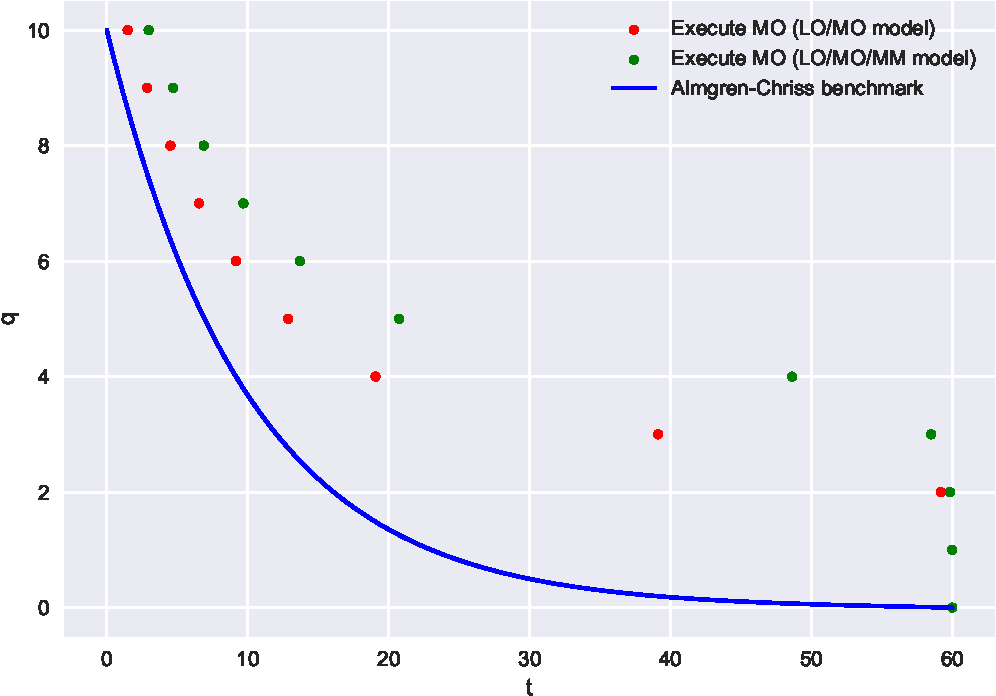
\includegraphics[width=0.9\textwidth]{marketorder.pdf}
  \caption{Optimal execution schdule and MO timing}
  \label{fig:mo}  
\end{figure}

\begin{table}[H]
  \centering
  \caption{Optimal MO execution timing}
  \label{tab:MO}
  \begin{tabular}{c|ccccccccccc} % 13列
  $q$ & 10 & 9 & 8 & 7 & 6 & 5 & 4 & 3 & 2 & 1 & 0 \\
  \hline
  $\tau_{\text{LO/MO}}$ & 1.47 & 2.86 & 4.51 & 6.54 & 9.17 & 12.87 & 19.07 & 39.12 & 59.19 & 59.99 & 60.00 \\
  $\tau_{\text{LO/MO/MM}}$ & 2.96 & 4.71 &	6.87 & 9.69	& 13.70	& 20.74	& 48.63	& 58.50	& 59.83	& 60.00	& 60.00 \\
  \end{tabular}
\end{table}

Table \ref{tab:zeta} shows the optimal market order execution size. 
Notice that in the LO/MO/MM model, the market order size 
$\zeta$ was also chosen optimally. 
$\zeta$ is a function of $t$ and $q$, and here it represents the statistics for the sample of 
$q=0$ to $10$ at each $t=10 - 50$. 
According to this, there is a trend that the execution size of the market order increases as time progresses. 
This can be attributed to the increasing need to complete the execution using the MO, 
even if the price is not as favorable as the LO or MM, due to the diminishing time remaining. 
Since market impact is incorporated as the $0.5$ power of the execution size, 
it is considered more efficient to execute 2 units in one MO rather than executing 1 unit twice."
\begin{table}[H]
  \centering
  \caption{Statistics of Optimal market order size of LO/MO/MM model}\label{tab:zeta}
  \begin{tabular}{|c|c|c|c|c|c|c|c|c|}
  \hline
  Time & count & mean & std & min & 25\% & 50\% & 75\% & max \\
  \hline
  10	& 11.0	& 0.545455	& 0.687552	& 0.0	& 0.0	& 0.0	& 1.0	& 2.0 \\
  20	& 11.0	& 0.909091	& 1.044466	& 0.0	& 0.0	& 1.0	& 1.5	& 3.0 \\
  30	& 11.0	& 1.272727	& 1.348400	& 0.0	& 0.0	& 1.0	& 2.0	& 4.0 \\
  40	& 11.0	& 1.272727	& 1.348400	& 0.0	& 0.0	& 1.0	& 2.0	& 4.0 \\
  50	& 11.0	& 1.545455	& 1.368476	& 0.0	& 0.5	& 1.0	& 2.5	& 4.0 \\
  \hline
  \end{tabular}
\end{table}

Table\ref{tab:delta_l}, \ref{tab:delta_i} and Figure \ref{fig:delta} shows, for Strategy 3, the optimal LO depth (dashed line) for each inventory at each time, 
as well as the optimal ask MM apread (solid line).
For simplicity in presentation, only the curves for odd inventory levels are shown here.
When comparing the LO depth $\delta^L$ and MM spread $\delta^I$ for the same inventory, 
they are nearly identical when there is still plenty of time remaining and the inventory is small around 1. 
On the other hand, when the remaining time is short and there is more inventory left, the MM spread is thinner than the LO depth (client-favorable) price, and it is particularly suggested that a better price can be offered, even beyond the mid.
This suggests that there is no market impact during execution through MM, and since execution can occur at a better price than the MO, even beyond the mid, this behavior aligns well with real-world experience.

\begin{table}[H]
  \centering
  \caption{LO depth}
  \label{tab:delta_l}
  \begin{tabular}{lccccc} % 左揃え（l）+ 中央揃え（c）で整形
  \hline
  $t$ & $\delta_t^{L*}(q=1)$ & $\delta_t^L(q=3)$ & $\delta_t^L(q=5)$ & $\delta_t^L(q=7)$ & $\delta_t^L(q=9)$ \\
  \hline
  10& 0.081970	& 0.029968	& 0.012390	& 0.004944	& 0.004944 \\
  20& 0.044861	& 0.015076	& 0.005066	& 0.004944	& 0.004944 \\
  30& 0.033752	& 0.011292	& 0.004944	& 0.004944	& 0.004822 \\
  40& 0.029480	& 0.009949	& 0.004944	& 0.004944	& 0.004822 \\
  50& 0.025574	& 0.008850	& 0.004944	& 0.004944	& 0.004822 \\
  \hline
  \end{tabular}
\end{table}


\begin{table}[H]
  \centering
  \caption{MM spread}
  \label{tab:delta_i}
  \begin{tabular}{lccccc} 
  \hline
  $t$ & $\delta_t^I(q=1)$ & $\delta_t^I(q=3)$ & $\delta_t^I(q=5)$ & $\delta_t^I(q=7)$ & $\delta_t^I(q=9)$ \\
  \hline
  10& 0.081992	& 0.029569	& 0.009957	&-0.000100  &-0.000100 \\
  20& 0.044826	& 0.013250	& 0.000050	&-0.000100  &-0.000100 \\
  30& 0.033527	& 0.008625	& -0.00010  &-0.000183 &-0.000237 \\
  40& 0.029097	& 0.006878	& -0.00010  &-0.000183 &-0.000237 \\
  50& 0.024879	& 0.005403	& -0.00010  &-0.000100 &-0.000280 \\
  \hline
  \end{tabular}
\end{table}

\begin{figure}[H]
  \centering
  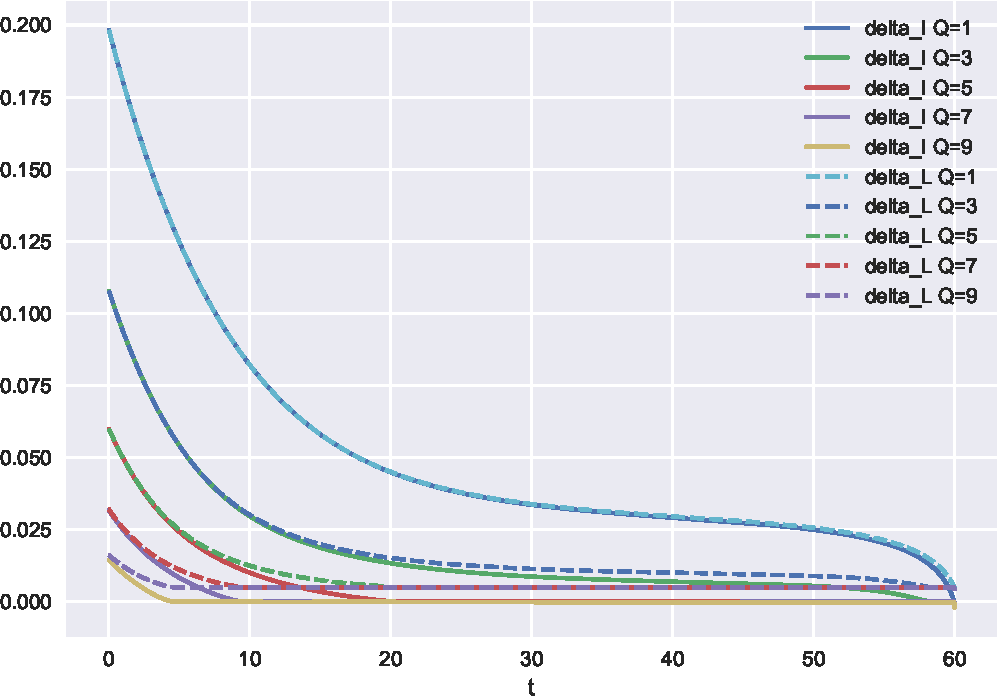
\includegraphics[width=0.9\textwidth]{delta_limitorder.pdf}
  \caption{Optimal spread $\delta^I$ and depth $\delta^L$}
  \label{fig:delta}  
\end{figure}

Table~\ref{tab:value_comparison} reports the reduced value function
$h(0,Q_0)$ obtained by solving the HJB-QVI backward in time.
Recall that the value function is decomposed as
\[
H(t,x,s,q)=x+qs+h(t,q),
\]
where $x$ denotes the cash position, $qs$ is the mark-to-market value
of the current inventory, and $h(t,q)$ represents the additional value
generated by optimally executing the remaining inventory from time $t$
onward.

In the comparison, we evaluate the value function at the normalized
initial state $(x,s,q)=(0,S_0,Q_0)$.
Since the cash component $x$ enters the value function additively and
the term $Q_0S_0$ is common across all models, the difference between
the models is entirely characterized by the reduced value function
$h(0,Q_0)$.
Therefore, comparing $h(0,Q_0)$ directly measures the difference in the
optimal expected execution value generated by each execution mechanism.

In the numerical example, the reduced value is
\[
h^{\mathrm{LO/MO}}(0,Q_0)=-0.041139,
\qquad
h^{\mathrm{LO/MO/MM}}(0,Q_0)=0.112355.
\]
The LO/MO benchmark produces a negative reduced value,
reflecting execution costs and inventory-risk penalties.
In contrast, the inclusion of internal market-making liquidity
turns the reduced value positive.
Hence, incorporating internal market-making liquidity improves the
reduced value by
\[
h^{\mathrm{LO/MO/MM}}(0,Q_0)
-
h^{\mathrm{LO/MO}}(0,Q_0)
=
0.153495.
\]
This positive difference indicates that the additional internal execution
channel increases the optimal value of the execution problem after
accounting for market-order costs, limit-order execution opportunities,
internal market-making executions, and inventory risk penalties.

\begin{table}[H]
\centering
\caption{Comparison of reduced value functions at the initial inventory}
\label{tab:value_comparison}
\begin{tabular}{lcc}
\hline
Strategy & Reduced value $h(0,Q_0)$ & Improvement over LO/MO \\
\hline
LO/MO    & $-0.041139$ & $0.000000$ \\
LO/MO/MM & $ 0.112355$ & $0.153495$ \\
\hline
\end{tabular}
\end{table}

Table~\ref{tab:sensitivity} and Figure~\ref{fig:sensitivity}
report sensitivity analyses of the reduced value function
with respect to the internal execution intensity $\lambda^I$,
the inventory penalty parameter $\phi$,
and the market-order impact parameter $\alpha^M$.

First, the reduced value of the LO/MO/MM model increases
monotonically as the internal execution intensity $\lambda^I$
increases, as shown in Figure~\ref{fig:sensitivity}(a).
This behavior is economically intuitive because a larger
$\lambda^I$ implies more frequent internal execution opportunities
through market making, allowing the agent to complete liquidation
with smaller market impact costs and reduced reliance on aggressive
market orders.
Consequently, the performance improvement over the benchmark
LO/MO model also increases monotonically.

Second, as the inventory penalty parameter $\phi$ increases,
the reduced values of both the LO/MO and LO/MO/MM models decrease,
as shown in Figure~\ref{fig:sensitivity}(b).
This is consistent with the interpretation of $\phi$
as a penalty for deviations from the benchmark liquidation trajectory.
A larger inventory penalty reduces the incentive to wait for favorable
executions through passive orders or internal liquidity,
leading to more immediate liquidation behavior.
As a result, the additional benefit obtained from internal
market-making liquidity becomes smaller as $\phi$ increases.

Finally, Figure~\ref{fig:sensitivity}(c) shows that the reduced value
exhibits only limited sensitivity with respect to the market-order
impact parameter $\alpha^M$ within the considered parameter range.
Although the reduced value decreases approximately linearly as
$\alpha^M$ increases, the magnitude of the variation remains relatively
small compared with the sensitivities to $\lambda^I$ and $\phi$.
This suggests that, under the optimal strategy,
market orders play a secondary role relative to limit-order and
internal executions, and are mainly used as a supplementary execution
mechanism near the terminal period.

Overall, the numerical results are consistent with the economic
intuition underlying the proposed model and support the effectiveness
of incorporating internal market-making liquidity into optimal
execution strategies.
In particular, the results indicate that the performance improvement
is primarily driven by the availability of internal liquidity itself,
rather than by the market-order mechanism.

\begin{table}[H]
\centering
\caption{Sensitivity analysis of the reduced value function}
\label{tab:sensitivity}
\begin{tabular}{llccc}
\hline
Parameter & Value & $H^{\mathrm{LO/MO}}(0)$ & $H^{\mathrm{LO/MO/MM}}(0)$ & Improvement \\
\hline

$\lambda^I$
& 0.333 & -0.041139 & 0.062264 & 0.103403 \\
& 0.667 & -0.041139 & 0.090276 & 0.131415 \\
& 1.000 & -0.041139 & 0.112355 & 0.153495 \\
& 1.333 & -0.041139 & 0.130370 & 0.171509 \\
& 1.667 & -0.041139 & 0.145538 & 0.186678 \\

\hline

$\phi$
& 0.00025 & -0.072251 & 0.147240 & 0.219491 \\
& 0.00050 & -0.056538 & 0.130043 & 0.186581 \\
& 0.00100 & -0.041139 & 0.112355 & 0.153495 \\
& 0.00200 & -0.023608 & 0.091985 & 0.115594 \\
& 0.00400 & -0.000898 & 0.065818 & 0.066716 \\

\hline

$\alpha^M$
& 0.000025 & -0.041139 & 0.112360 & 0.153500 \\
& 0.000050 & -0.041139 & 0.112358 & 0.153498 \\
& 0.000100 & -0.041139 & 0.112355 & 0.153495 \\
& 0.000200 & -0.041139 & 0.112349 & 0.153488 \\
& 0.000400 & -0.041139 & 0.112337 & 0.153477 \\

\hline
\end{tabular}
\end{table}

\begin{figure}[H]
\centering
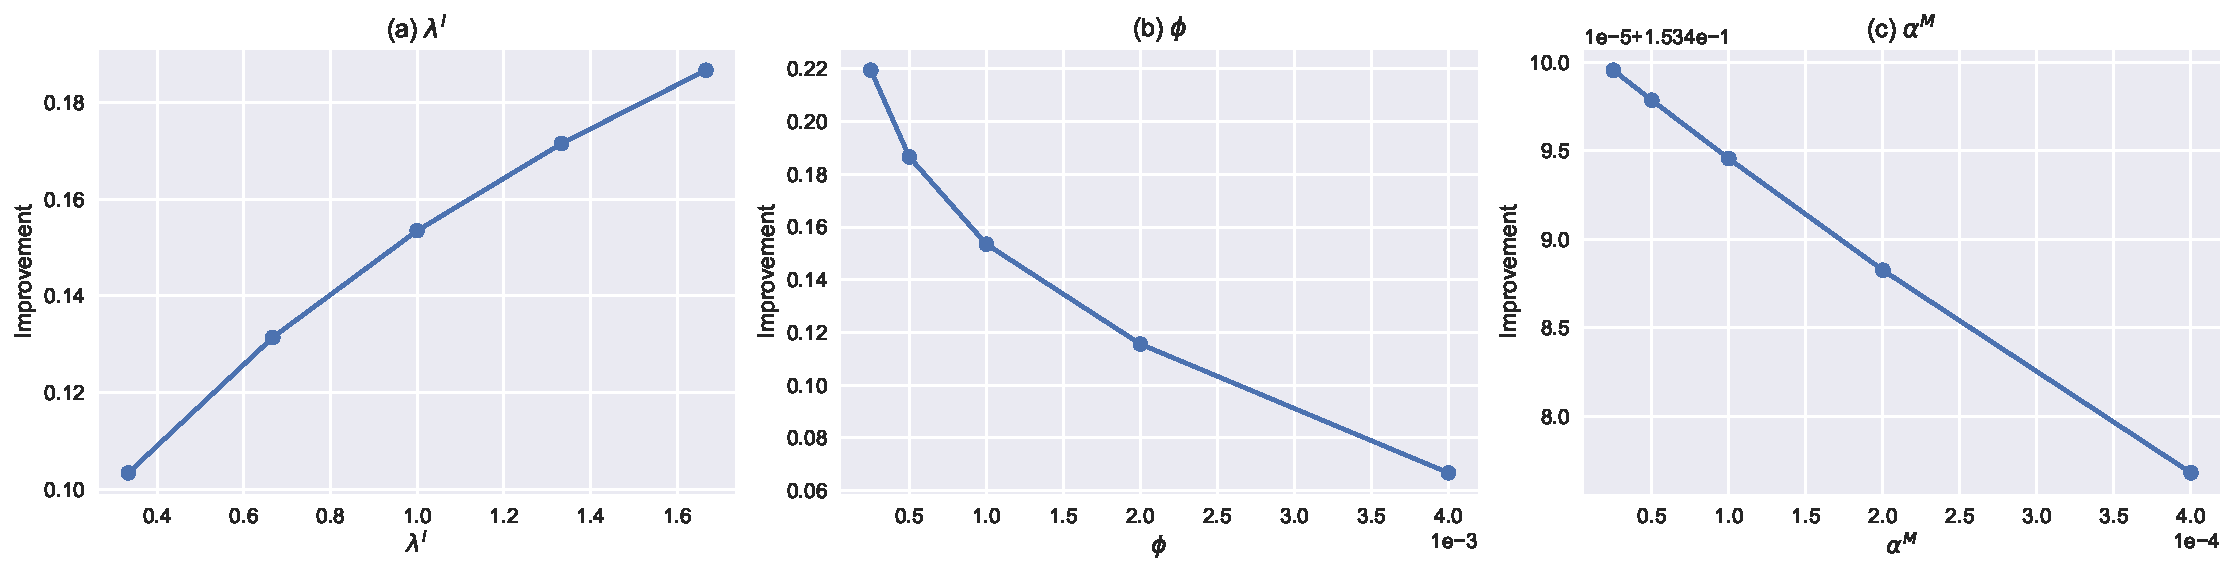
\includegraphics[width=\textwidth]{sensitivity_all.pdf}
\caption{
Sensitivity of the improvement over the LO/MO benchmark
with respect to
(a) internal execution intensity $\lambda^I$,
(b) inventory penalty parameter $\phi$,
and
(c) market-order impact parameter $\alpha^M$.
}
\label{fig:sensitivity}
\end{figure}

\bibliographystyle{plain}
\bibliography{references}  % references.bib を指定


\end{document}


